% !TeX root = SmithEmielBP.tex
%%=============================================================================
%% Gecontroleerde validatie
%%=============================================================================

\chapter{\IfLanguageName{dutch}{Gecontroleerde validatie}{Controlled validation}}%
\label{ch:validatie}

Hoofdstuk~\ref{ch:risicoanalyse} vertaalde de bevindingen uit de contextanalyse naar vijf onderzoekshypothesen. Dit hoofdstuk toetst deze hypothesen op een gecontroleerde en reproduceerbare manier. De bedoeling is niet om nieuwe willekeurige kwetsbaarheden te zoeken of de productieomgeving actief te belasten, maar om na te gaan in welke mate de eerder afgebakende risicocondities ook praktisch ondersteund worden door observaties, connectiviteitstesten, traceroutes, browsertests, passieve netwerkcaptatie en loggingcontrole.

De validatie vertrekt vanuit dezelfde afbakening als de voorgaande hoofdstukken. Individuele camera's worden niet als rechtstreeks internet-exposed systemen behandeld. De nadruk ligt op de beheerhost, TruVision Navigator, de NVR, de router/default gateway, de tussenliggende netwerkcomponenten, de bereikbaarheid van beheer- en applicatiediensten en de mate waarin uitgevoerde acties achteraf detecteerbaar zijn. De resultaten worden per hypothese beoordeeld als bevestigd, gedeeltelijk bevestigd of niet bevestigd, conform de acceptatiecriteria uit Hoofdstuk~\ref{ch:risicoanalyse}.

\section{\IfLanguageName{dutch}{Validatieopzet en bewijsvoering}{Validation setup and evidence collection}}%
\label{sec:validatie-opzet}

De technische validatie werd uitgevoerd vanuit een host op het beheer-/wifi-segment van De Rore. Deze testhost had tijdens de metingen het IP-adres \texttt{10.0.0.156}. De router/default gateway en DNS-server binnen dit segment was \texttt{10.0.0.150}. De NVR was bereikbaar op \texttt{10.0.0.60}. De gekende camera-adressen bevinden zich in het bereik \texttt{192.168.0.10} tot en met \texttt{192.168.0.26}, terwijl tijdens de metingen ook een tussenliggende component op \texttt{192.168.0.212} werd waargenomen.

De gebruikte aanpak bleef bewust niet-invasief. Er werden geen destructieve tests uitgevoerd, geen onbeperkte brute-forcepogingen gedaan en er werden geen configuratiewijzigingen aangebracht aan de productieomgeving. De bewijsvoering bestaat uit een combinatie van commandoregeloutput, browsertests, passieve netwerkobservaties, screenshots van beheerinterfaces en controle van beschikbare logs. Tabel~\ref{tab:validatie-bewijsbronnen} geeft een overzicht van de belangrijkste bewijsbronnen per hypothese.

\begin{table}[htbp]
    \centering
    \small
    \caption[Bewijsbronnen per hypothese]{Gebruikte bewijsbronnen per hypothese binnen de gecontroleerde validatie.}
    \label{tab:validatie-bewijsbronnen}
    \begin{tabular}{p{0.12\textwidth}p{0.31\textwidth}p{0.46\textwidth}}
        \hline
        \textbf{Hypothese} & \textbf{Focus} & \textbf{Belangrijkste bewijsbronnen} \\
        \hline
        H1 & Authenticatie en accountbeheer & Observatie van gedeelde adminaccounts, afwezige functiescheiding, wachtwoordcontext en beheerpraktijk. \\
        H2 & Segmentatie en laterale bereikbaarheid & \texttt{ipconfig}, \texttt{ping}, \texttt{tracert}, bereikbaarheid van \texttt{10.0.0.60}, \texttt{10.0.0.150}, \texttt{192.168.0.212} en camera-adressen. \\
        H3 & Beheer- en streamingdiensten & \texttt{Test-NetConnection}, browsertests naar beheerinterfaces, poortbereikbaarheid en observaties rond HTTP/HTTPS, RTSP en NVR-poorten. \\
        H4 & Remote access en externe publicatie & Installatiefiche, DynDNS-validatie, \texttt{nslookup}, externe \texttt{Test-NetConnection}-tests naar poorten \texttt{8000} en \texttt{8888}. \\
        H5 & Logging en detecteerbaarheid & Screenshot van de controlehistoriek, logcategorieën, succesvolle loginregistratie, exportmogelijkheid en interviewinformatie over opvolging. \\
        \hline
    \end{tabular}
\end{table}

\section{\IfLanguageName{dutch}{H1: Authenticatie en accountbeheer}{H1: Authentication and account management}}%
\label{sec:h1-authenticatie}

Hypothese H1 stelt dat zwakke of onvoldoende unieke credentials op de NVR, de beheerhost of cameracomponenten kunnen leiden tot ongeautoriseerde toegang tot beheer- of consultatiefuncties. Deze hypothese werd niet getest via agressieve authenticatiepogingen, maar via een gecontroleerde beoordeling van de aanwezige accountstructuur en de manier waarop toegang in de praktijk georganiseerd is.

Uit de contextanalyse bleek dat zowel op de Windows-beheerhost als binnen TruVision Navigator gewerkt wordt met een gedeeld adminaccount. Daardoor ontbreekt persoonlijke toewijzing van acties aan individuele gebruikers. Hetzelfde beheerprincipe keert terug in de camerabeheeromgeving, waar het onderscheid tussen gewone raadpleging en administratief beheer beperkt is. Bovendien wordt de beveiliging in sterke mate gedragen door één enkele authenticatiefactor, zonder multifactorauthenticatie of duidelijke functiescheiding.

De belangrijkste vaststelling is niet enkel dat één wachtwoord zwak of contextgebonden kan zijn, maar vooral dat de volledige beheerketen afhankelijk is van gedeelde, hooggeprivilegieerde toegang. Wanneer meerdere personen dezelfde adminidentiteit gebruiken, wordt het moeilijk om achteraf te bepalen wie welke handeling uitvoerde. Daarnaast betekent kennis of compromittering van één credential meteen toegang tot brede beheerfunctionaliteit.

\paragraph{Beoordeling.}
H1 wordt als \textbf{gedeeltelijk bevestigd} beoordeeld. De onderliggende risicoconditie is duidelijk aanwezig: er is sprake van gedeelde adminaccounts, beperkte accountability, ontbrekende functiescheiding en geen multifactorauthenticatie. Tegelijk zijn in de huidige bewijsset geen afzonderlijke testartefacten opgenomen die aantonen dat beperkte authenticatieproeven effectief tot ongeautoriseerde toegang hebben geleid. De hypothese is dus sterk ondersteund op configuratie- en procesniveau, maar niet volledig empirisch bewezen via een afzonderlijke toegangstest.

\paragraph{Implicatie.}
Voor de verdere mitigatiefase betekent dit dat persoonlijke accounts, gescheiden rollen, sterkere wachtwoordvereisten en waar mogelijk aanvullende authenticatiemaatregelen prioritair moeten worden behandeld. Deze maatregelen verminderen niet alleen de kans op misbruik, maar verbeteren ook traceerbaarheid en verantwoordelijkheid bij beheerhandelingen.

\section{\IfLanguageName{dutch}{H2: Netwerksegmentatie en laterale bereikbaarheid}{H2: Network segmentation and lateral reachability}}%
\label{sec:h2-segmentatie}

Hypothese H2 onderzoekt of de bestaande netwerkstructuur laterale beweging vanuit of naar de camerazone voldoende beperkt. De oorspronkelijke aanname van een volledig vlak netwerk werd tijdens de contextanalyse reeds genuanceerd. De NVR bevindt zich op \texttt{10.0.0.60}, terwijl de camera's in de \texttt{192.168.0.x}-range geadresseerd zijn. Daardoor was al duidelijk dat de beheercomponent en de individuele camera's niet noodzakelijk in hetzelfde IP-segment zitten.

De metingen bevestigen deze nuance. Een traceroute naar de NVR op \texttt{10.0.0.60} eindigde rechtstreeks bij dit adres. Een traceroute naar \texttt{192.168.0.212} verliep via de router/default gateway \texttt{10.0.0.150} en bereikte daarna \texttt{192.168.0.212}. Een traceroute naar camera \texttt{192.168.0.15} bereikte daarentegen niet rechtstreeks de camera, maar eindigde met een \textit{Destination host unreachable}-melding afkomstig van \texttt{192.168.0.212}. Ook pingresultaten ondersteunen dit beeld: de NVR en \texttt{192.168.0.212} waren bereikbaar, terwijl een individuele camera vanuit het onderzochte segment niet rechtstreeks bereikbaar bleek.

{\small
    \begin{verbatim}
        tracert 192.168.0.212
        1  10.0.0.150
        2  192.168.0.212
        
        tracert 192.168.0.15
        1  10.0.0.150
        2  169.254.11.21
        3  192.168.0.212 reports: Destination host unreachable.
    \end{verbatim}
}

Deze resultaten tonen dat de omgeving niet volledig vlak is. Er bestaat minstens een vorm van routering of laag-3-scheiding tussen het beheer-/wifi-segment en het cameragerelateerde segment. Tegelijk betekent dit niet automatisch dat de segmentatie ook als volwaardige beveiligingsmaatregel kan worden beschouwd. De router/default gateway op \texttt{10.0.0.150} en de component op \texttt{192.168.0.212} bleven vanuit het onderzochte segment bereikbaar. Bovendien boden deze componenten beheerinterfaces aan, waardoor het aanvalsoppervlak niet beperkt blijft tot de camera's zelf.

\paragraph{Beoordeling.}
H2 wordt als \textbf{gedeeltelijk bevestigd} beoordeeld. De oorspronkelijke stelling van een volledig vlak netwerk moet worden bijgestuurd: er is wel degelijk een vorm van netwerkstructurering aanwezig. Tegelijk is de bestaande scheiding niet voldoende aangetoond als sterke beveiligende segmentatie, omdat tussenliggende beheercomponenten en beheerpaden bereikbaar blijven vanuit het onderzochte segment.

\paragraph{Implicatie.}
De belangrijkste implicatie is dat De Rore niet enkel nood heeft aan verschillende IP-ranges, maar aan expliciete toegangsregels tussen zones. Segmentatie moet niet alleen logisch bestaan, maar ook afdwingen welke hosts welke beheerinterfaces, NVR-diensten en cameracomponenten mogen bereiken.



\section{\IfLanguageName{dutch}{H3: Actieve beheer- en streamingdiensten}{H3: Active management and streaming services}}%
\label{sec:h3-diensten}

Hypothese H3 stelt dat actieve beheer- of streamingdiensten, zoals HTTP, RTSP of ONVIF, het interne aanvalsoppervlak vergroten wanneer ze onvoldoende afgeschermd zijn. De validatie focuste daarom op feitelijke bereikbaarheid van diensten vanuit de testhost op \texttt{10.0.0.156}, met aandacht voor beheerinterfaces, transportbeveiliging en het verschil tussen documentair aanwezige protocolondersteuning en effectief bereikbare diensten.

De resultaten tonen dat de dienstblootstelling niet homogeen is. Op \texttt{10.0.0.150} en \texttt{192.168.0.212} waren de poorten \texttt{80} en \texttt{443} bereikbaar. Via de browser werd telkens een loginpagina waargenomen. HTTPS was technisch aanwezig of geadverteerd, maar de observaties wijzen erop dat HTTP-toegang niet volledig werd uitgesloten. Voor de NVR op \texttt{10.0.0.60} waren de poorten \texttt{8000} en \texttt{8888} bereikbaar. De poorten \texttt{80}, \texttt{443} en \texttt{554} waren vanuit het onderzochte segment niet bereikbaar.

\begin{table}[htbp]
    \centering
    \small
    \caption[Samenvatting van bereikbare diensten tijdens de validatie]{Samenvatting van bereikbare diensten vanuit de testhost \texttt{10.0.0.156}.}
    \label{tab:validatie-poorten}
    \begin{tabular}{p{0.22\textwidth}p{0.22\textwidth}p{0.43\textwidth}}
        \hline
        \textbf{Host} & \textbf{Bereikbare poorten} & \textbf{Interpretatie} \\
        \hline
        \texttt{10.0.0.150} & \texttt{80}, \texttt{443} & Router/default gateway met bereikbare webbeheerinterface. HTTP-toegang werd waargenomen. \\
        \texttt{192.168.0.212} & \texttt{80}, \texttt{443} & Downstream of gerouteerde component met bereikbare webinterface. \\
        \texttt{10.0.0.60} & \texttt{8000}, \texttt{8888} & NVR-gerelateerde applicatie- of beheerpoorten bereikbaar vanuit het beheer-/wifi-segment. \\
        \texttt{10.0.0.60} & \texttt{554} niet bereikbaar & RTSP op de NVR werd vanuit dit segment niet bevestigd. \\
       Camera-adressen &
       Niet rechtstreeks bereikbaar &
       Ping vanaf de testhost naar \texttt{192.168.0.15} gaf \textit{Destination host unreachable} met antwoord van \texttt{192.168.0.212}; rechtstreekse bereikbaarheid van individuele camera's werd dus niet aangetoond. \\
        \hline
    \end{tabular}
\end{table}

Deze bevindingen tonen dat het relevante aanvalsoppervlak zich vanuit het onderzochte segment vooral situeert op de beheerketen en de NVR, niet op rechtstreeks bereikbare camerawebinterfaces. De aanwezigheid van RTSP en ONVIF blijft op basis van inventarisatie en werking van de cameraketen aannemelijk, maar werd vanuit deze testpositie niet rechtstreeks op cameraniveau gevalideerd. Dat onderscheid is belangrijk: H3 wordt niet bevestigd omdat alle camera's breed toegankelijk zouden zijn, maar omdat kritieke beheer- en recordertoegang intern bereikbaar blijven en minstens één beheerpad via HTTP kon worden benaderd.

\paragraph{Beoordeling.}
H3 wordt als \textbf{gedeeltelijk bevestigd} beoordeeld. Meerdere beheergerelateerde diensten zijn intern actief en bereikbaar op kritieke componenten. Tegelijk konden RTSP- en ONVIF-blootstelling op individuele camera's vanuit het onderzochte segment niet rechtstreeks worden gevalideerd. De hypothese wordt dus ondersteund voor beheer- en NVR-diensten, maar blijft genuanceerd voor rechtstreekse cameraprotocollen.

\paragraph{Implicatie.}
De belangrijkste implicatie is dat beheerinterfaces en NVR-poorten expliciet moeten worden afgeschermd. Het uitschakelen of beperken van onnodige diensten, het afdwingen van HTTPS, het beperken van beheerinterfaces tot specifieke beheerhosts en het controleren van RTSP/ONVIF-bereikbaarheid blijven belangrijke mitigatiedomeinen.


\section{\IfLanguageName{dutch}{H4: Externe publicatie en remote access}{H4: External publication and remote access}}%
\label{sec:h4-remote-access}

Hypothese H4 onderzoekt of externe toegang tot de NVR of tot netwerkcomponenten die toegang tot het cameradomein ontsluiten, onvoldoende afgeschermd is. De validatie werd bewust niet opgevat als een agressieve internettest van individuele camera's. De focus lag op de historisch gedocumenteerde remote-accessroute en op de interne bereikbaarheid van beheerpaden die toegang tot de camerainfrastructuur kunnen ondersteunen.

De installatiefiche vermeldt een DynDNS-hostname in combinatie met poort \texttt{8888}. Een actuele DNS-controle toonde aan dat \texttt{derore01.dyndns.org} nog resolveerde naar een publiek IP-adres. Daarna werd met \texttt{Test-NetConnection} gecontroleerd of de poorten \texttt{8000} en \texttt{8888} via deze hostname bereikbaar waren. Beide TCP-tests faalden op het testmoment.

{\small
    \begin{verbatim}
        nslookup derore01.dyndns.org
        Name:    derore01.dyndns.org
        Address: 141.135.202.68
        
        Test-NetConnection derore01.dyndns.org -Port 8000
        TcpTestSucceeded : False
        
        Test-NetConnection derore01.dyndns.org -Port 8888
        TcpTestSucceeded : False
    \end{verbatim}
}

Deze resultaten moeten voorzichtig geïnterpreteerd worden. De DNS-validatie toont dat de historische DynDNS-verwijzing nog bestaat op DNS-niveau, maar de mislukte TCP-verbinding toont niet aan dat de NVR op het testmoment publiek bereikbaar was via poort \texttt{8888}. Tegelijk werden de actuele NAT-, port-forwarding-, VPN- en firewallregels niet rechtstreeks ingezien. Er kan dus niet sluitend worden vastgesteld of de remote-accessketen volledig uitgeschakeld, afgeschermd of op een andere manier gewijzigd is.

Naast de externe controle tonen de interne metingen dat meerdere relevante beheerpaden vanuit het beheer-/wifi-segment bereikbaar zijn. Het gaat onder meer om de webinterface op \texttt{10.0.0.150}, een bijkomende component op \texttt{192.168.0.212} en NVR-poorten op \texttt{10.0.0.60}. Daardoor ligt het risico niet uitsluitend bij aantoonbare publieke internetblootstelling, maar ook bij historisch voorziene remote-accesspaden en intern bereikbare beheerdiensten.

\paragraph{Beoordeling.}
H4 wordt als \textbf{gedeeltelijk bevestigd} beoordeeld. Remote access was historisch voorzien en de DynDNS-hostname resolveert nog, maar actuele publieke TCP-bereikbaarheid van de onderzochte poorten werd niet aangetoond. Wel blijven interne beheerpaden en NVR-gerelateerde poorten bereikbaar vanuit een intern of semibevoorrecht segment.

\paragraph{Implicatie.}
Voor de mitigatiefase betekent dit dat remote access expliciet geïnventariseerd en herbeoordeeld moet worden. Port forwarding, VPN-configuratie, DynDNS-gebruik en firewallregels moeten aantoonbaar gedocumenteerd zijn. Beheertoegang op afstand hoort enkel beschikbaar te zijn via een sterk afgeschermd mechanisme met minimale blootstelling.


\section{\IfLanguageName{dutch}{H5: Logging en detecteerbaarheid}{H5: Logging and detectability}}%
\label{sec:h5-logging}

Hypothese H5 onderzoekt of uitgevoerde acties binnen de camerabeheeromgeving voldoende zichtbaar worden in logs en of die logging bruikbaar is voor detectie en reconstructie. De initiële aanname was dat logging mogelijk beperkt bleef tot een kleine set aan login- of exportevents. De observaties tonen echter een genuanceerder beeld.

In TruVision Navigator is een controlehistoriek aanwezig met meerdere filtercategorieën. De interface toont onder meer categorieën voor inloggen, uitloggen, configuratiewijziging, video downloaden, momentopname exporteren, uitgang activeren, firmware uploaden, databaseback-up, database herstellen en machtiging wijzigen. Binnen de getoonde periode werd minstens één succesvolle aanmelding geregistreerd: een \textit{Logon}-event van het account \texttt{Admin} op \texttt{2026-04-13 10:12:33}, met als detail dat de gebruiker ingelogd is.

Deze vaststelling toont dat de omgeving niet loggingloos is. De beheerapplicatie ondersteunt meerdere auditcategorieën en registreert minstens basisinformatie zoals gebeurtenistype, tijdstip, bron, gebruikersnaam en detailomschrijving. Tegelijk is de operationele waarde van deze logging beperkt of minstens onvoldoende aangetoond. Uit de beschikbare gegevens blijkt niet dat logs centraal verzameld worden, automatisch gecorreleerd worden of aanleiding geven tot waarschuwingen. Uit de interviewinformatie blijkt bovendien dat logs zelden tot nooit actief gecontroleerd worden, dat er geen e-mailwaarschuwingen worden verstuurd bij verdachte acties en dat opvolging in de praktijk bij de zaakvoerders ligt.

\paragraph{Beoordeling.}
H5 wordt als \textbf{gedeeltelijk bevestigd en inhoudelijk verfijnd} beoordeeld. De oorspronkelijke aanname dat logging zeer beperkt of bijna afwezig zou zijn, moet worden genuanceerd: er is wel degelijk een bredere applicatieve controlehistoriek aanwezig. Tegelijk blijft de centrale bezorgdheid overeind dat deze logging vooral reactief en lokaal bruikbaar lijkt, zonder aangetoonde centrale monitoring, correlatie of proactieve alerting.

\paragraph{Implicatie.}
De belangrijkste implicatie is dat logging niet alleen aanwezig moet zijn, maar ook actief gebruikt moet worden als detectiemechanisme. Voor De Rore betekent dit dat logretentie, export, periodieke controle, waarschuwingen bij kritieke events en duidelijke verantwoordelijkheden rond opvolging moeten worden uitgewerkt.


\begin{figure}[H]
         \centering
         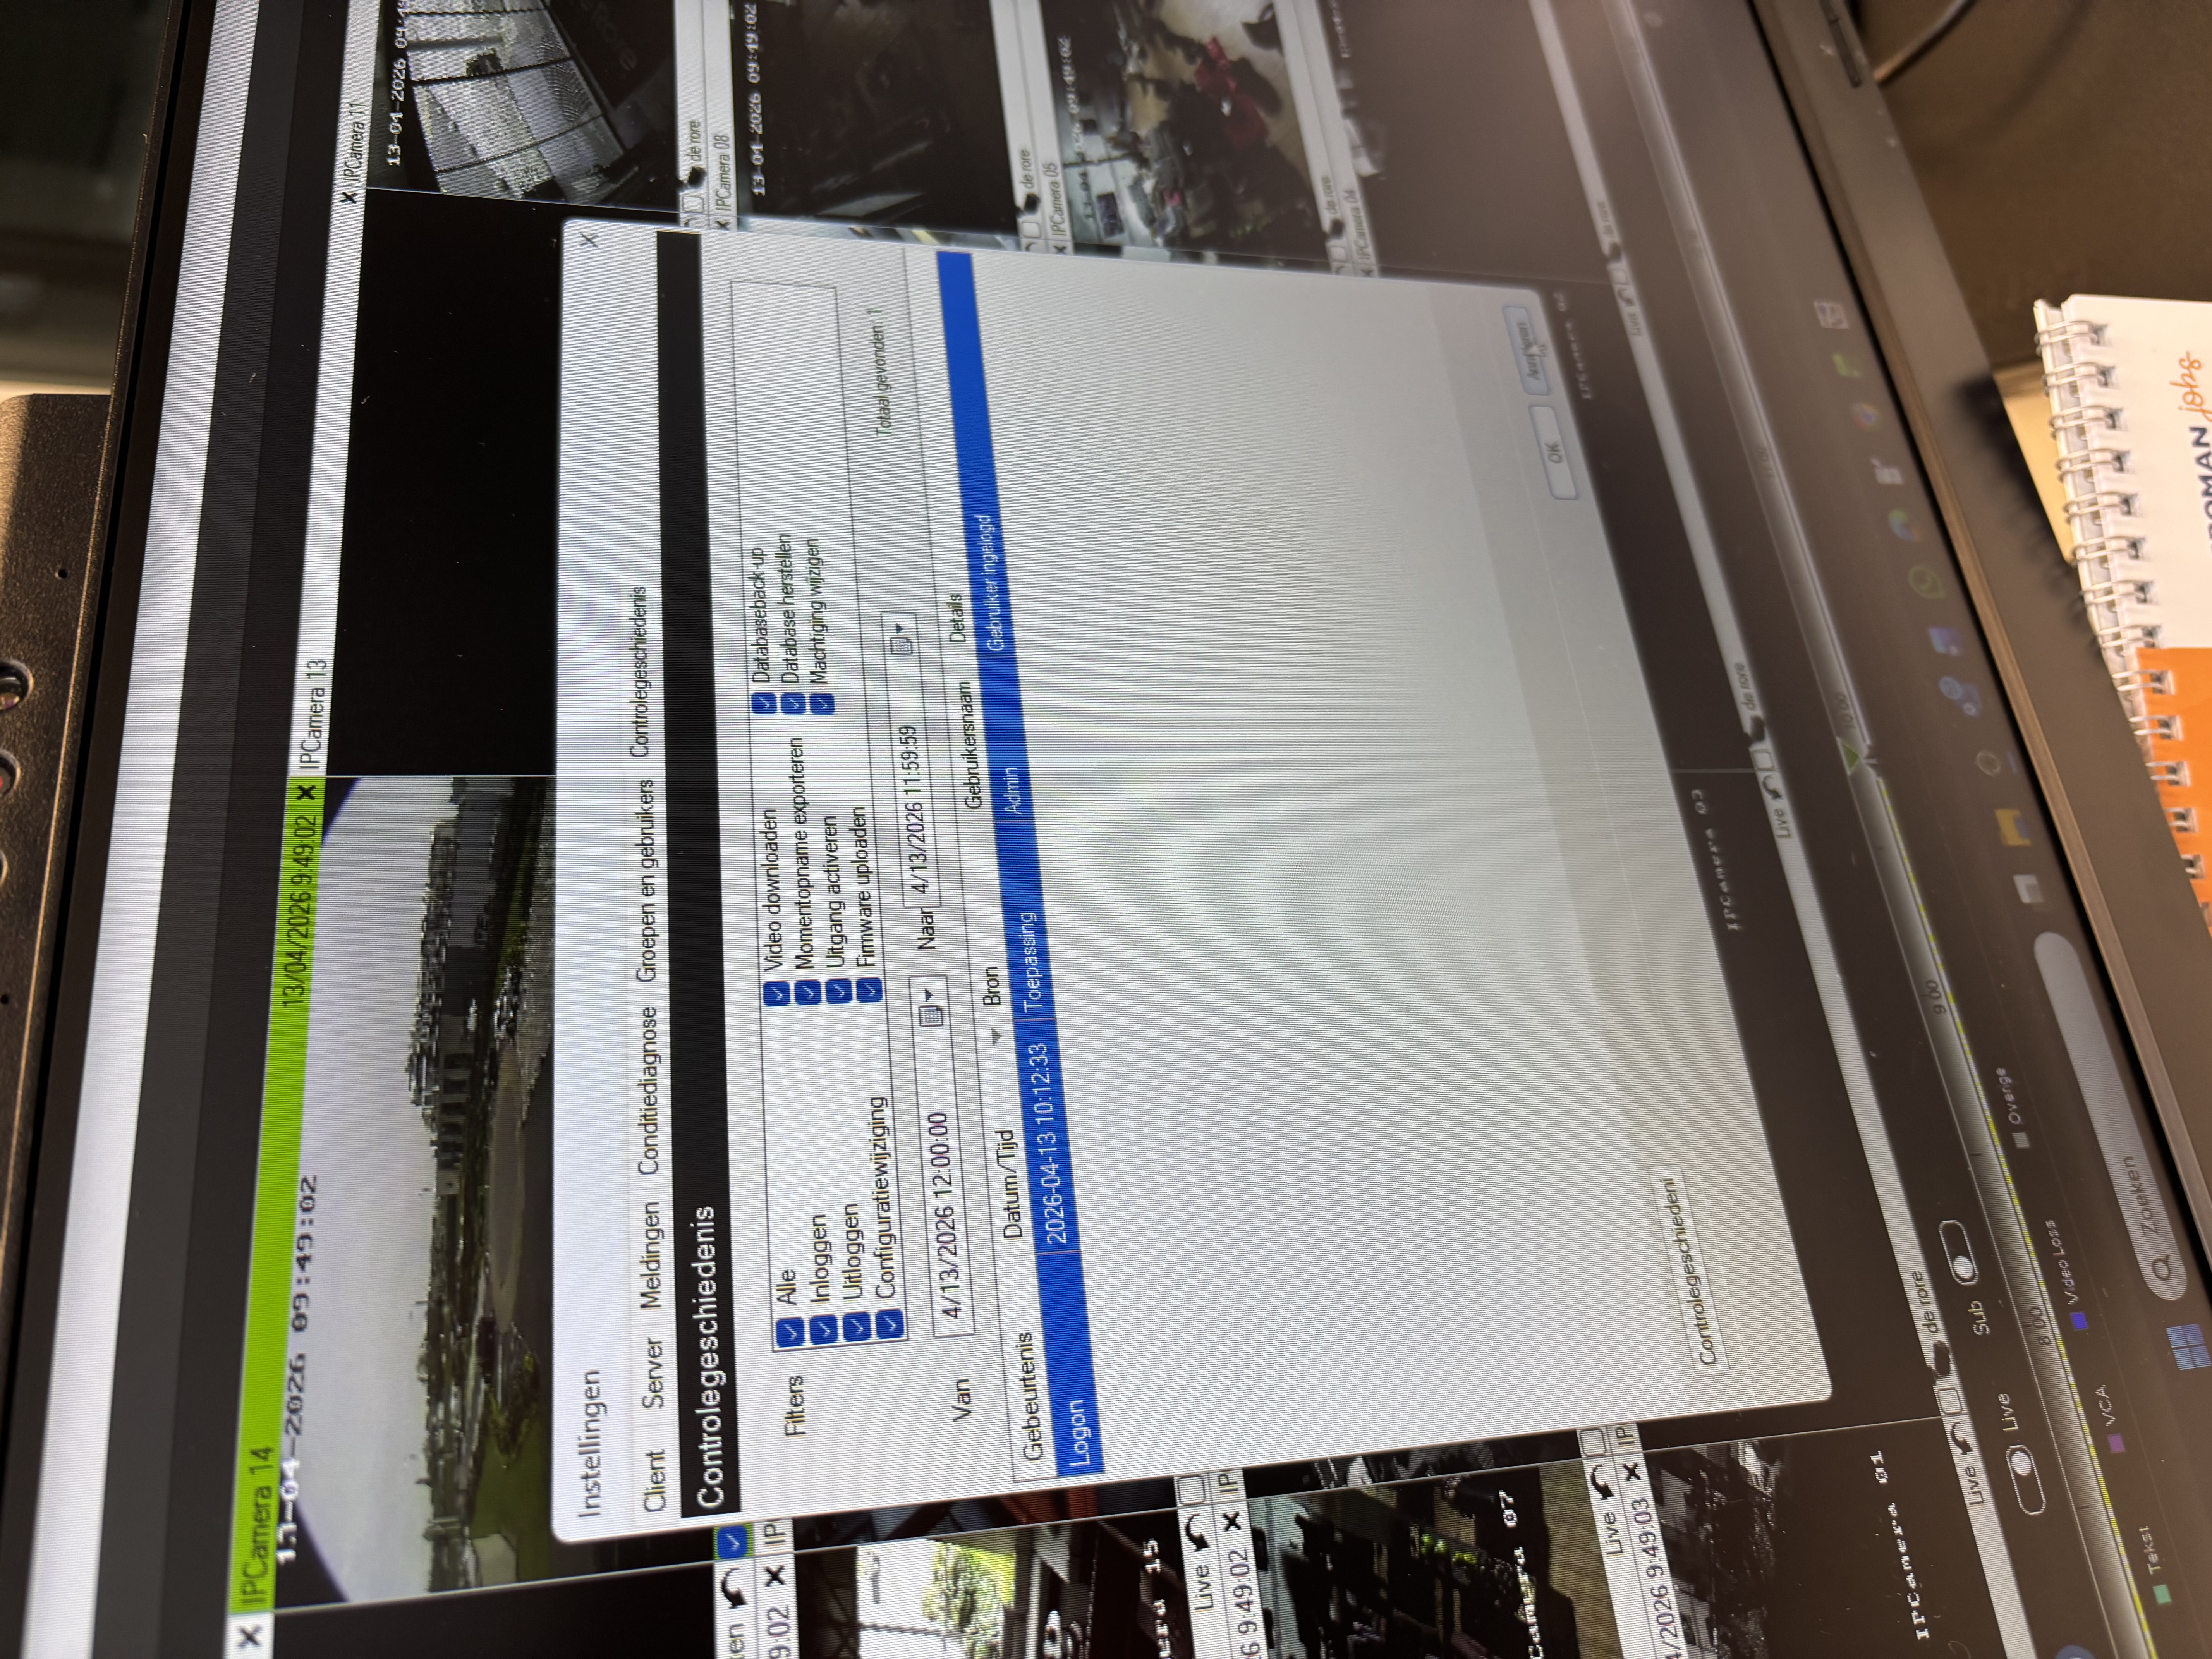
\includegraphics[angle=-90,width=.85\textwidth]{../Voorbereiding/Bewijsstukken/H1/logging_controlehistoriek}
         \caption[Controlehistoriek in TruVision Navigator]{Voorbeeld van de controlehistoriek in TruVision Navigator met logcategorieën en een geregistreerde succesvolle aanmelding.}
         \label{fig:controlehistoriek-truvision}
     \end{figure}

\section{\IfLanguageName{dutch}{Synthese van de validatie}{Validation synthesis}}%
\label{sec:validatie-synthese}

De gecontroleerde validatie toont dat de belangrijkste risico's binnen de camerainfrastructuur van De Rore niet louter theoretisch zijn. De resultaten bevestigen tegelijk dat de oorspronkelijke aannames moeten worden verfijnd. De omgeving is niet volledig vlak en de individuele camera's bleken vanuit het onderzochte segment niet rechtstreeks bereikbaar. Toch blijven meerdere beheerpaden, NVR-poorten en tussenliggende beheercomponenten intern bereikbaar. Ook op het vlak van logging blijkt de situatie genuanceerder dan aanvankelijk gedacht: er is meer logging aanwezig dan verwacht, maar de maturiteit als detectiemechanisme blijft beperkt.

Tabel~\ref{tab:synthese-validatie} vat de beoordeling per hypothese samen.

\begin{table}[htbp]
    \centering
    \small
    \caption[Synthese van de validatie per hypothese]{Synthese van de validatie per hypothese.}
    \label{tab:synthese-validatie}
    \begin{tabular}{p{0.10\textwidth}p{0.27\textwidth}p{0.18\textwidth}p{0.35\textwidth}}
        \hline
        \textbf{Hyp.} & \textbf{Risicothema} & \textbf{Beoordeling} & \textbf{Kernbevinding} \\
        \hline
        H1 & Authenticatie en accountbeheer & Gedeeltelijk bevestigd & Gedeeld adminaccount, beperkte functiescheiding en geen MFA; geen afzonderlijke exploitvalidatie. \\
        H2 & Segmentatie en laterale bereikbaarheid & Gedeeltelijk bevestigd & Niet volledig vlak netwerk, maar tussenliggende componenten en beheerpaden blijven bereikbaar. \\
        H3 & Beheer- en streamingdiensten & Gedeeltelijk bevestigd & Beheerinterfaces en NVR-poorten zijn bereikbaar; RTSP/ONVIF op cameraniveau niet rechtstreeks gevalideerd. \\
        H4 & Remote access en externe publicatie & Gedeeltelijk bevestigd & DynDNS bestaat nog op DNS-niveau; publieke TCP-bereikbaarheid niet aangetoond; interne beheerpaden wel bereikbaar. \\
        H5 & Logging en detecteerbaarheid & Gedeeltelijk bevestigd en verfijnd & Controlehistoriek bestaat, maar actieve monitoring, alerting en centrale correlatie zijn niet aangetoond. \\
        \hline
    \end{tabular}
\end{table}

De zwaarste aandachtspunten situeren zich op drie niveaus. Ten eerste blijft identiteits- en toegangsbeheer kwetsbaar door gedeelde adminaccounts en beperkte functiescheiding. Ten tweede is de netwerkarchitectuur slechts gedeeltelijk afgeschermd: er zijn verschillende segmenten, maar de praktische toegangsbeperking tussen beheeromgeving, NVR en cameradomein is niet volledig aangetoond. Ten derde zijn meerdere beheer- en applicatiediensten intern bereikbaar, terwijl logging vooral reactief lijkt en niet aantoonbaar als proactieve detectielaag functioneert.

Deze validatie vormt de directe basis voor Hoofdstuk~\ref{ch:threatmodel}. In dat hoofdstuk worden de gevalideerde en genuanceerde bevindingen gestructureerd via STRIDE en vertaald naar concrete mitigatiemaatregelen voor De Rore. De nadruk verschuift daarbij van de vraag welke risico's aanwezig zijn naar de vraag welke dreigingsscenario's daaruit volgen en welke maatregelen de grootste risicoreductie opleveren binnen een realistische KMO- en retailcontext.
